\subsection{Lab19: Modulación QPSK - Transmision y recepcion}

%*********************
\begin{frame}{}

\pgfdeclareimage[width=\paperwidth,height=\paperheight]{bg}{imagenes/fondo_lab}
\setbeamertemplate{background}{\pgfuseimage{bg}}

\bfseries{\textrm{ \Large Lab 19: \\Modulación QPSK - Transmisión y Recepción}}
\raggedright
\end{frame}
%********************

%--------------------------------------------------------------------------------------------
\begin{frame}{Modulación QPSK - Transmisión y Recepción}

\pgfdeclareimage[width=\paperwidth,height=\paperheight]{bg}{imagenes/fondo3}
\setbeamertemplate{background}{\pgfuseimage{bg}}

\justifying
Este ejercicio mostrará la modulación y demodulación digital QPSK en GRC donde se enviara información en formato .txt y .jpg, estos datos seran modulados en QPSK y luego transmitidos mediante un virtual sink, seguido de esto seran recepcionados mediante un virtual source, en donde estos seran demodulados para poder visualizarlos en un nuevo archivo de recepción. 

\end{frame}
%---------------------------------------------------------------------------
%\includegraphics[scale=1]{../imagenes/descarga.jpeg} 
\begin{frame}{Modulación QPSK - Transmisión y Recepción}
\begin{figure}
\includegraphics[scale=.4]{Modulaciones_digitales/lab19/pdf/lab19_1.pdf}
\end{figure}
\end{frame}
%--------------------------------------------------------------------------------------
\begin{frame}{Modulación QPSK - Transmisión y Recepción}
\begin{figure}
\includegraphics[scale=.4]{Modulaciones_digitales/lab19/pdf/lab19_2.pdf}
\end{figure}
\end{frame}

%---------------------------------------------------------------------------------------

\begin{frame}{Modulación QPSK - Transmisión y Recepción}
	\justifying
	La definición de la constelación en el bloque Constellation Object se efectua de acuerdo a la cantidad de símbolos posibles en la misma dentro del espacio complejo o el diagrama de constelación. Para la constelación de QPSK se manejan 4 símbolos, entonces de acuerdo a la siguiente ecuación los bits para cada símbolo serían 2.\\
	\centering
	$\log_{2}(4)=2$ bits/símbolo\\
	\begin{figure}
		\includegraphics[scale=.4]{Modulaciones_digitales/lab19/pdf/lab19_4.pdf}
	\end{figure}
\end{frame}

%-----------------------------------------------------------------------------------

\begin{frame}{Modulación QPSK - Transmisión y Recepción}
	\begin{figure}
		\includegraphics[scale=.35]{Modulaciones_digitales/lab19/pdf/lab19_2_1.pdf}
	\end{figure}
\end{frame}

%-----------------------------------------------------------------------------------
\begin{frame}{Modulación QPSK - Transmisión y Recepción}
	\justifying
	Este el resultado al transmitir datos mediante la modulación QPSK, cabe resaltar que el tiempo de transmisión de los datos varia dependiendo del tamaño del archivo, es por esto que se debe esperar un cierto tiempo para la transmisión completa. 
	\begin{figure}
		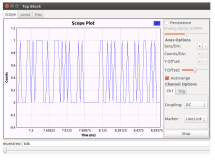
\includegraphics[scale=.4]{Modulaciones_digitales/lab19/pdf/lab19_3.pdf}
	\end{figure}
\end{frame}
%---------------------------------------------------------------------------
\begin{frame}{Modulación QPSK - Transmisión y Recepción}
\justifying
Constelación QPSK con codificación diferencial habilitada y 4 Muestras por símbolo
\begin{figure}
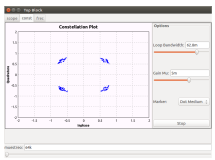
\includegraphics[scale=.4]{Modulaciones_digitales/lab19/pdf/lab19_5.pdf}
\end{figure}
\end{frame}
%-------------------------------------------------------------------------------------------
